% lark-eunis16.tex
% 

\ifdefined\handout         % ----- IEEE HPEC conference proceedings

\documentclass[ignorenonframetext,handout]{beamer}

\else

\documentclass[ignorenonframetext]{beamer}

\fi

% -------------------- PREAMBLE

% ----- customizations

% preamble-packages.tex


% fix booktabs compatibility issue
\usepackage{etex}
\usepackage{animate}

% math
\usepackage{sansmathaccent}
\usepackage{amsmath}
\usepackage{amssymb}
\usepackage{mathrsfs}
\usepackage{array}


% graphics
\usepackage[font=small,compatibility=false,justification=centering]{caption}
\usepackage[font=small,labelformat=empty,justification=centering]{subcaption}
\usepackage{graphicx}
\usepackage{tikz}

\usepackage{dirtree}

% tables
\usepackage{multirow}
\usepackage{booktabs}

% fonts
\usepackage{natbib}
\usepackage{todonotes}

\usepackage{textpos}

\usepackage{microtype}

\usepackage{grffile}

% for Android theme
\usepackage{bold-extra}
\usepackage{listings}


% directory path
\usepackage{menukeys}

%%% Local Variables:
%%% mode: latex
%%% TeX-master: "../android-studio-main"
%%% End:

% preamble-extras.tex
%
%

\usetheme[bullet=circle,% Use circles instead of squares for bullets.
          titleline=true,% Show a line below the frame title.
          alternativetitlepage=true,% Use the fancy title page.
          titlepagelogo=figs/android-logo,% Logo for the first page.
          watermark=figs/android-watermark,% Watermark used in every page.
          watermarkheight=100px,% Height of the watermark.
          watermarkheightmult=4,% The watermark image is 4 times bigger
                                % than watermarkheight.
          ]{Android}


\lstset{language=Java,captionpos=b,
tabsize=4,frame=lines,
basicstyle=\scriptsize\ttfamily,
keywordstyle=\color{blue},
commentstyle=\color{lightgray},
stringstyle=\color{violet},
breaklines=true,showstringspaces=false}

\AtBeginSection[]{%
  \begin{frame}<beamer>
    \frametitle{Outline}
    \tableofcontents[currentsection]
  \end{frame}
  \addtocounter{framenumber}{-1}% If you don't want them to affect the slide number
}



%%% Local Variables:
%%% mode: latex
%%% TeX-master: "../android-studio-main"
%%% End:
% preamble-customizations.tex


% fix Linux Adobe Acrobat Reader's issue with transparent image elements
% \pdfpageattr{/Group << /S /Transparency /I true /CS /DeviceRGB>>}


% define coloured clickable links
\hypersetup{%
  pdffitwindow=false,%
  pdfstartview={FitH},%
  % colorlinks,%
  pdfauthor={},%
  pdftitle={},%
  pagebackref=true,%
  citecolor=PaleGreen4,%
  filecolor=DarkOrchid4,%
  % linkcolor=OrangeRed4,%
  urlcolor=RoyalBlue4%
}

% define the includegraphics search path
\graphicspath{%
  {figs/}%
}

% short-hand command for hyperlinked e-mails
\newcommand{\email}[1]{\href{mailto:#1}{\texttt{#1}}}

% redefine \boxed command to allow setting the border color
\newcommand{\highlight}[1]{\fcolorbox{complclr1}{white}{$\displaystyle #1$}}

% modified bullet-point for highlighting
\newcommand{\bulletemph}{$\large\boldsymbol{\star}$}

% command to output names under images
\newcommand{\imentry}[3][1.25cm]{%
  \vbox{\halign{\hfil##\hfil\cr%
      \includegraphics[height=#1]{#2}\cr#3\cr}}}

\definecolor{custom_theme}{HTML}{91043D}

%%% Local Variables:
%%% mode: latex
%%% TeX-master: "../android-studio-main"
%%% End:


\sloppy

% ---------- DATE
% 

\newcommand{\datestring}{Mar. 20, 2017}
\date%
[\datestring]%
{\footnotesize \datestring}

% ---------- TITLE
%
\title%
[Android Studio Development]%
{ Android Development using Android Studio% \\
  % \emph{Learning with Computer-Assisted Guided Tours}%
}


% ---------- CONFERENCE
%
\subtitle%
{ \footnotesize BEST Mobile App Development }



% ---------- AUTHORS
%
\author%
[D. Floros]%
{%
  \imentry{dimitris-floros.png}{Dimitris Floros} \and%
}


% ---------- AFFILIATIONS
\institute%
[]%
{%
  Department of Electrical and Computer Engineering,
  Aristotle University of Thessaloniki%
}



% -------------------- MAIN MATTER

\begin{document}
\frame[plain]{\titlepage}

\frame{\tableofcontents[]}

\mode<all>

%---- INTRODUCTION --------

\section{Introduction}
\label{sec:introduction}

% general introduction
% introduction.tex
%
%

\begin{frame}
  \frametitle{What is Android?}
  
  \begin{itemize}
    
  \item<1-> Android represents an exciting new oppurtinity to write
    innovative applications for smartphones
  \item<2-> Android is an \emph{open-source} stack that includes
    \begin{itemize}
    \item<3-> Operating system
    \item<3-> Middleware
    \item<3-> API libraries
    \end{itemize}
    
  \item<3-> Powered by Linux operating system

  \item<4-> Fast application development in Java

  \end{itemize}

\end{frame}



%%% Local Variables:
%%% mode: latex
%%% TeX-master: "../android-studio-main"
%%% End:


% android devices possibilities
% android-devices.tex
%
%

\begin{frame}
  \frametitle{Android devices}
  
  Modern mobile smart-phones have become powerful tools

  \begin{itemize}
  \item<2-> Cameras
  \item<3-> WiFi -- 4G
  \item<4-> GPS system
  \item<5-> Sensors
    \begin{itemize}
    \item<6-> Accelerometer
    \item<6-> Gyroscope
    \item<6-> Magnetometer
    \end{itemize}
  \end{itemize}
  
  \onslide<7->{
    New possibilities in \emph{application development}
  }

\end{frame}

%%% Local Variables:
%%% mode: latex
%%% TeX-master: "../android-studio-main"
%%% End:

%  LocalWords:  Accelerometer


% ---------- ANDROID PLATFORM

\section{Android Platform Architecture}
\label{sec:android-platform}

% image showing Android stack
% android-stack.tex
%
%


\begin{frame}[plain]

  \begin{figure}
    \centering
    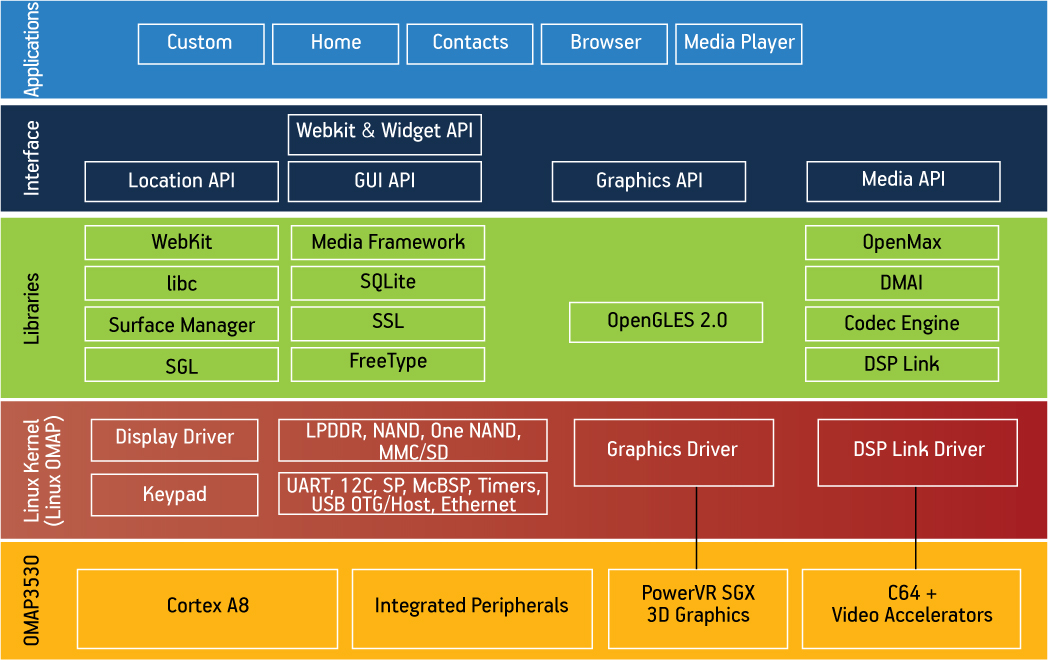
\includegraphics[height=0.8\textheight]{android-application-stack}
    \caption{Android Software Stack on OMAP3530 \\
      \emph{Source}: Texas Instruments}
    \label{fig:android-stack}
  \end{figure}
  
\end{frame}


%%% Local Variables:
%%% mode: latex
%%% TeX-master: "../android-studio-main"
%%% End:


% linux kernel
% linux-kernel.tex
%
%


\begin{frame}
  \frametitle{Linux Kernel}
  
  \begin{itemize}
  \item<1-> Works as a HAL (Hardware Abstraction Layer)
  \item<2-> Device drivers
  \item<3-> Memory management
  \item<4-> Process management
  \item<5-> Networking
  \end{itemize}

  \begin{figure}
    \centering
    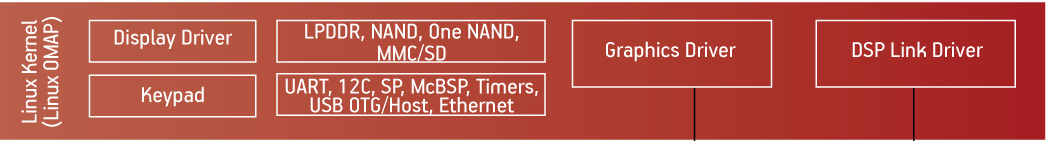
\includegraphics[width=\textwidth]{android-application-stack-linux-kernel}
  \end{figure}


\end{frame}


%%% Local Variables:
%%% mode: latex
%%% TeX-master: "../android-studio-main"
%%% End:


% libraries
% libraries.tex
%
%


\begin{frame}
  \frametitle{Libraries}
  
  \begin{itemize}
  \item<1-> C/C++ libraries
  \item<2-> Interface through Java
  \item<3-> Surface manager -- Handling UI Windows
  \item<4-> 2D and 3D graphics
  \item<5-> Media codecs, SQLite, Browser engine
  \end{itemize}

  \begin{figure}
    \centering
    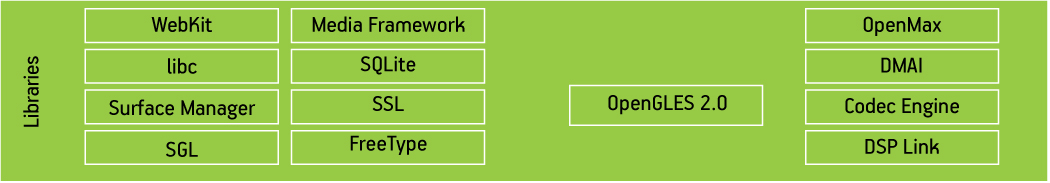
\includegraphics[width=\textwidth]{android-application-stack-libraries}
  \end{figure}


\end{frame}


%%% Local Variables:
%%% mode: latex
%%% TeX-master: "../android-studio-main"
%%% End:


% interface
% interface.tex
%
%


\begin{frame}
  \frametitle{Applications}
  
  \begin{itemize}
  \item<1-> API interface
  \item<2-> Access to libraries through Java
  \end{itemize}

  \begin{figure}
    \centering
    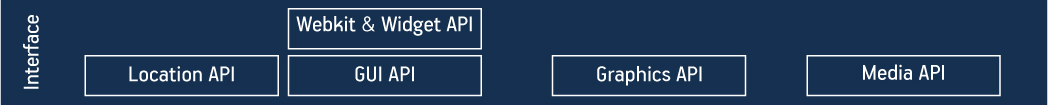
\includegraphics[width=\textwidth]{android-application-stack-interface}
  \end{figure}

  \onslide<3->{%
    \emph{This level is important for application development --
      Provides interface to the underlying libraries}
  }%

\end{frame}


%%% Local Variables:
%%% mode: latex
%%% TeX-master: "../android-studio-main"
%%% End:


% applications
% applications-layer.tex
%
%


\begin{frame}
  \frametitle{Interface}
  
  \begin{itemize}
  \item<1-> Built in and user applications
  \item<2-> The level where our applications are developed
  \end{itemize}

  \begin{figure}
    \centering
    
\includegraphics[width=\textwidth]{android-application-stack-applications}
  \end{figure}

\end{frame}


%%% Local Variables:
%%% mode: latex
%%% TeX-master: "../android-studio-main"
%%% End:


% ---------- BUILDING BLOCKS

\section{Building Blocks}
\label{sec:building-blocks}

% android building blocks
% android-building-blocks.tex
%
%


\begin{frame}[plain]
  
  \begin{figure}
    \centering
    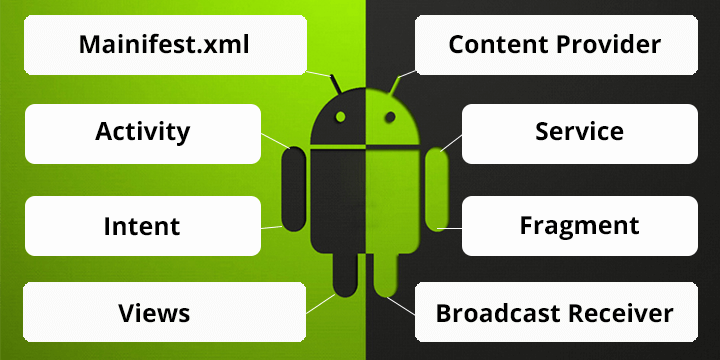
\includegraphics[width=\textwidth]{android-building-blocks}
    \caption{Android building blocks \\
      \emph{Source}: \url{www.programmersnight.com}}
    \label{fig:android-stack}
  \end{figure}
  
\end{frame}


%%% Local Variables:
%%% mode: latex
%%% TeX-master: "../android-studio-main"
%%% End:


% activity
%
%
%

\begin{frame}
  \frametitle{Activity}
  
  \begin{itemize}
  \item<1-> Entry point for interacting with the user
  \item<2-> An application can have multiple activities
  
  \item<2->[] For example an email app can have the following activities 
    \begin{itemize}
    \item Show emails
    \item Compose email
    \item Read email
    \end{itemize}
        
  \item<4-> Keeps track of what the user currently cares about

  \end{itemize}

\end{frame}


%%% Local Variables:
%%% mode: latex
%%% TeX-master: "../android-studio-main"
%%% End:


% lifecycle
% android-stack.tex
%
%


\begin{frame}[plain]

  \begin{figure}
    \centering
    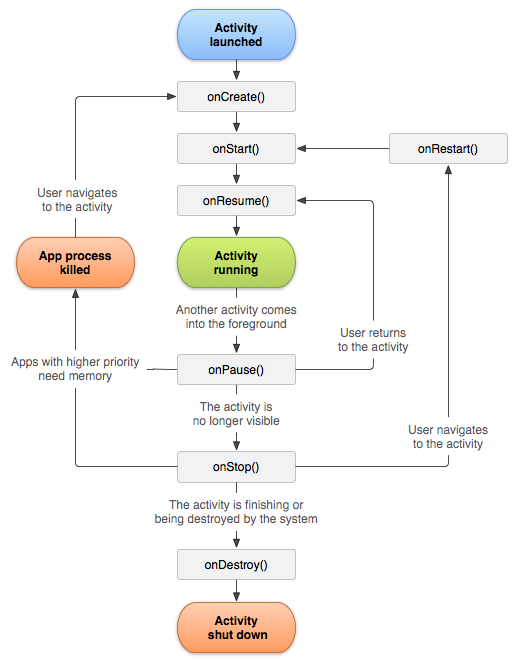
\includegraphics[height=0.9\textheight]{activity-lifecycle}
    \caption{A simplified illustration of the activity lifecycle \\
      \emph{Source}:\url{developer.android.com}}
    \label{fig:android-lifecycle}
  \end{figure}
  
\end{frame}


%%% Local Variables:
%%% mode: latex
%%% TeX-master: "../android-studio-main"
%%% End:


% intent
% intent-block.tex
%
%

\begin{frame}
  \frametitle{Intents}
  
  \begin{itemize}
  \item<1-> Used to invoke components
  
  \item<2->[] Mainly used to 
    \begin{itemize}
    \item<3-> Start a service
    \item<4-> Launch an activity
    \item<5-> Display a web page
    \item<6-> Broadcast a message
    \item<7-> Dial a phone call
    \end{itemize}
    
  \item<8-> Enables one application to start a component of a
    different one

  \item<9-> A different application can start whichever one
  \item<9->[] (as long as the other app allows it)


  \end{itemize}

\end{frame}


%%% Local Variables:
%%% mode: latex
%%% TeX-master: "../android-studio-main"
%%% End:


% views
% views-block.tex
%
%

\begin{frame}
  \frametitle{Views}
  
  \begin{itemize}
  \item<1-> Anything you see is a view
  
  \item<2->[] A view can contain multiple UI elements
    \begin{itemize}
    \item<3-> Buttons
    \item<4-> Labels
    \item<5-> Text fields
    \item<6-> Search bar
    \item<7-> Images
    \end{itemize}
    
  \item<8-> The layout is designed in \texttt{XML}

  \item<9-> Views along with resources are separate from source code.

  \end{itemize}

\end{frame}


%%% Local Variables:
%%% mode: latex
%%% TeX-master: "../android-studio-main"
%%% End:


% service
% service-block.tex
%
%

\begin{frame}
  \frametitle{Service}
  
  \begin{itemize}
  \item<1-> General purpose entry point for keeping an app running in
    the background
  
  \item<2-> Does not provide user interface

  \item<3-> A service might play music in the background while the
    user is in a different app

  \item<4-> Another component can start the service and 

    \begin{itemize}
    \item<4-> Let it run
    \item<4-> Bind to it for interaction
    \end{itemize}

  \item<5-> Two different types of services

    \begin{itemize}
    \item<6-> Foreground with a notification
    \item<7-> Background without notification
      \begin{itemize}
      \item<7-> The user is not directly aware
      \item<7-> Can be killed by the system if it needs \texttt{RAM}
      \end{itemize}
    \end{itemize}

  \end{itemize}

\end{frame}


%%% Local Variables:
%%% mode: latex
%%% TeX-master: "../android-studio-main"
%%% End:


% broadcast receiver
% broadcast-receiver-block.tex
%
%

\begin{frame}
  \frametitle{Broadcast receiver}
  
  \begin{itemize}
  \item<1-> Enables the system to deliver events to the app outside of
    regular user flow
  
  \item<2-> Respond to system-wide broadcast announcements

  \item<3-> System can deliver broadcast even to apps not currently running
    \begin{itemize}
    \item<4-> An app can schedule an alarm to post a notification
      informing the user of an upcoming event
    \item<5-> By delivering as a Broadcast receiver, the app does not
      need to remain running
    \end{itemize}
    
    
  \item<6-> System broadcasts

    \begin{itemize}
    \item<6-> Low battery
    \item<6-> Screen off
    \end{itemize}

    
  \item<7-> Most commonly is used as a gateway to other components
  \item<8-> Intended for minimal work

  \end{itemize}

\end{frame}


%%% Local Variables:
%%% mode: latex
%%% TeX-master: "../android-studio-main"
%%% End:


% manifest
% manifest-block.tex
%
%

\begin{frame}
  \frametitle{Manifest}
  
  \begin{itemize}
  \item<1-> Declares an applications available components
  
  \item<2-> Identifies any user permissions the app requires
    
  \item<3-> Declares the minimum \texttt{API} level required
  
  \item<4-> Hardware \& software features used or required

  \item<5-> \texttt{API} libraries needed to be linked against

  \end{itemize}

\end{frame}


%%% Local Variables:
%%% mode: latex
%%% TeX-master: "../android-studio-main"
%%% End:


% ---------- ANDROID STUDIO

\section{Android Studio}
\label{sec:android-studio}

% what is android studio
% android-studio.tex
%
%


\begin{frame}[plain]
  \frametitle{Android Studio}

  \begin{figure}
    \centering
    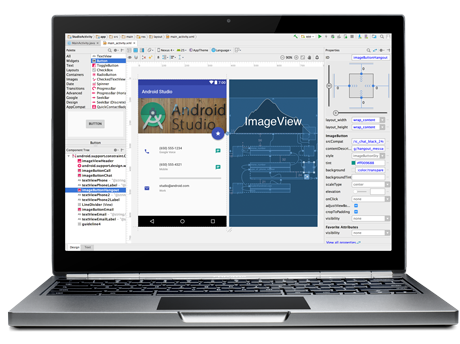
\includegraphics[height=0.8\textheight]{android-studio-home}
    \caption{Android Studio \\
      \emph{Source}: \url{developer.android.com}}
    \label{fig:android-studio-home}
  \end{figure}
  
\end{frame}

\begin{frame}
  \frametitle{Android Studio}
  \framesubtitle{Introduction}

  \begin{itemize}
  \item<1-> Available for free
  \item<2-> Cross-platform (Windows, Linux, MacOS)
  \item<3-> Based on \texttt{Intellij IDEA IDE}
  \end{itemize}

\end{frame}


\begin{frame}
  \frametitle{Android Studio}
  \framesubtitle{Build system}

  \begin{itemize}
  \item<1-> Gradle build system
  \item<2-> Easy configuration of projects
  \item<3-> Include code libraries
  \item<4-> Generate multiple build variants
  \item<5-> Robust dependency management
  \end{itemize}

\end{frame}


\begin{frame}
  \frametitle{Android Studio}
  \framesubtitle{Multiple Android device}

  \begin{itemize}
  \item<1-> Unified environment for
    \begin{itemize}
    \item<2-> Android phones
    \item<3-> Android tables
    \item<4-> Android Wear
    \item<5-> Android TV
    \item<6-> Android Auto
    \end{itemize}
  \item<7-> Target multiple form factors with single project
  \item<8-> Share code among different versions
  \end{itemize}

\end{frame}

%%% Local Variables:
%%% mode: latex
%%% TeX-master: "../android-studio-main"
%%% End:


% ---------- HELLO ANDROID

\section{Hello Android Application}
\label{sec:hello-android}

% create new project
% create-new-project.tex
%
%

\begin{frame}
  \frametitle{New project}
  
  
  \begin{itemize}
  \item<1-> In \texttt{Android Studio} click \texttt{Start a new Android
      Studio project}

  \item<2-> Enter \texttt{Application Name} and \texttt{Company
      Domain}
    
  \item<3-> Keep default \texttt{Target Android Devices}

  \item<4-> Select \texttt{Empty Activity}

  \item<5-> Finish

  \end{itemize}


\end{frame}



%%% Local Variables:
%%% mode: latex
%%% TeX-master: "../android-studio-main"
%%% End:


% important files
% important-files.tex
%
%

\begin{frame}
  \frametitle{Important files}
  
  After processing, \texttt{Android Studio} opens the \texttt{IDE}.  

  Let us review the most important files

  \begin{itemize}
  \item<1-> \directory{app/java/com.example.myfirstapp/MainActivity.java}
    
    \begin{itemize}
    \item<1-> Main activity
    \item<1-> Entry point for application
    \end{itemize}

  \item<2-> \directory{app/res/layout/activity\_main.xml}
    
    \begin{itemize}
    \item<2-> Layout of activity's UI
    \item<2-> Contains \texttt{TextView} with the text ''Hello world!''
    \end{itemize}

  \item<3-> \directory{app/manifests/AndroidManifest.xml}
    
    \begin{itemize}
    \item<3-> Describes fundamental characteristics of the app
    \item<3-> Declares each component -- permissions -- API library
    \end{itemize}

  \item<4-> \directory{Gradle Scripts/build.gradle}

    \begin{itemize}
    \item<4-> Automate and manage build process
    \end{itemize}

  \end{itemize}

\end{frame}

%%% local Variables:
%%% mode: latex
%%% TeX-master: "../android-studio-main"
%%% End:
 

% how to create an activity
% activity-creation.tex
%
%


\begin{frame}
  \frametitle{Creating an Activity}
  \framesubtitle{Part 1}

  \begin{itemize}
  \item<1-> To create an activity, you must create a subclass of
    \texttt{Activity}

  \item<2-> In your class you need to implement \texttt{callback
      methods}

    \begin{itemize}
    \item<3-> \lstinline{onCreated()}
    \item<4-> \lstinline{onPause()}
    \item<5-> \lstinline{onStopped()}
    \item<6-> \lstinline{onResumed()}
    \item<7-> \lstinline{onDestroyed()}
    \end{itemize}
  \end{itemize}

\end{frame}


\begin{frame}
  \frametitle{Creating an Activity}
  \framesubtitles{Part 2}

  
  \begin{itemize}
  \item<1-> \lstinline{onCreated()}

    \begin{itemize}
    \item<2-> Called when created
    \item<3-> Initialization done here
    \end{itemize}

  \item<4-> \lstinline{onPause()}

    \begin{itemize}
    \item<5-> Called when user leaves activity
    \item<6-> Commit persistent changes
    \end{itemize}

  \end{itemize}

\end{frame}


%%% Local Variables:
%%% mode: latex
%%% TeX-master: "../android-studio-main"
%%% End:


% user interface
% user-interface.tex
%
%

\begin{frame}
  \frametitle{User interface}
  \framesubtitle{Views}


  \begin{itemize}
  \item<1-> User interface is provided by a hierarchy of views objects
  \item<2-> Each view controls a particular space within the activity
    window
  \item<3-> For example, a view might be a text box to write a message
  \end{itemize}

\end{frame}

\begin{frame}
  \frametitle{User interface}
  \framesubtitle{Layouts}


  \begin{itemize}
  \item<1-> Provide a unique layout model for child view
  \item<2-> The most common way to define a layout is with an \texttt{XML}
  \item<3-> You can set the layout for an activity with
    \lstinline{setContentView()}
  \end{itemize}

\end{frame}


%%% Local Variables:
%%% mode: latex
%%% TeX-master: "../android-studio-main"
%%% End:


% declaring activity in manifest
% manifest-declare-activity
%
%

\begin{frame}[fragile]
  \frametitle{Manifest}
  \framesubtitle{Declare activity}
  
  You must declare your activity in the manifest file

  \begin{exampleblock}{Example}
    
\begin{lstlisting}
<manifest ... >
  <application ... >
    <activity android:name=".ExampleActivity" />
        ...
  </application ... >
  ...
</manifest>
\end{lstlisting}


  \end{exampleblock}

\end{frame}


\begin{frame}[fragile]
  \frametitle{Manifest}
  \framesubtitle{Use intent filters}
  
  Declare how other application components may activate it

  \begin{exampleblock}{Example}
\begin{lstlisting}
<activity android:name=".ExampleActivity" android:icon="@drawable/app_icon">
    <intent-filter>
        <action android:name="android.intent.action.MAIN" />
        <category android:name="android.intent.category.LAUNCHER" />
    </intent-filter>
</activity>
\end{lstlisting}
  \end{exampleblock}

\end{frame}

%%% Local Variables:
%%% mode: latex
%%% TeX-master: "../android-studio-main"
%%% End:


% starting an activity
% starting-an-activity.tex
%
%

\begin{frame}[fragile]
  \frametitle{Starting an Activity}
  

  You need to pass an \texttt{Intent} during the call to
  \lstinline{startActivity()} that describes the activity you want to
  start

  \begin{exampleblock}{Example}
\begin{lstlisting}
Intent intent = new Intent(this, SignInActivity.class);
startActivity(intent);
\end{lstlisting}
  \end{exampleblock}

  You can shutdown an activity by its \lstinline{finish()} method

\end{frame}

%%% Local Variables:
%%% mode: latex
%%% TeX-master: "../android-studio-main"
%%% End:


% views and inflation
% views-example.tex
%
%

\begin{frame}[fragile]
  \frametitle{Views}
  \framesubtitle{Inflating activity layout}

  To display a user interface you need to assign a View to an Activity

\begin{lstlisting}
@Override
public void onCreate(Bundle bundle) {
    super.onCreate(bundle);
    setContentView(R.layout.main);
    TextView textView = (TextView)findViewById(R.id.textView);
}
\end{lstlisting}


\end{frame}


\begin{frame}[fragile]
  \frametitle{Views}
  \framesubtitle{Event listeners}

  \begin{itemize}
  \item<1-> Java event handling mechanism
  \item<2-> Interfaces containing methods that are invoked on some
    user action
  \end{itemize}

  \begin{exampleblock}{\texttt{OnClickListener}}
\begin{lstlisting}
private OnClickListener btnClicked = new OnClickListener() {
    public void onClick(View v) {
        // do something when button is clicked
    }
};
protected void onCreate(Bundle bundle) {
    // Capture our button from layout
    Button btn = (Button) findViewById(R.id.btn);
    // Register the onClick listener with the implementation above
    btn.setOnClickListener(btnClicked);
}
\end{lstlisting}
  \end{exampleblock}

\end{frame}

%%% Local Variables:
%%% mode: latex
%%% TeX-master: "../android-studio-main"
%%% End:


% online resources
% online-resources.tex
%
%

\begin{frame}
  \frametitle{Online resources}
  
  \begin{itemize}
  \item<1-> Android Developers
    \begin{itemize}
    \item \url{http://developer.android.com}
    \end{itemize}
  \item<2-> Android Studio -- SDK
    \begin{itemize}
    \item \url{http://developer.android.com/sdk/index.html}
    \end{itemize}
  \item<3-> Google Play Store
    \begin{itemize}
    \item \url{ https://play.google.com/store }
    \end{itemize}
  \end{itemize}

\end{frame}

%%% Local Variables:
%%% mode: latex
%%% TeX-master: "../android-studio-main"
%%% End:



% ---------- ACKNOWLEDGMENTS

% \section*{Acknowledgments}
% acknowledgment.tex
%
%
%

\begin{frame}[plain]
  \frametitle{Acknowledgment}
  \begin{tabular}{cl}  
    \begin{tabular}{c}
      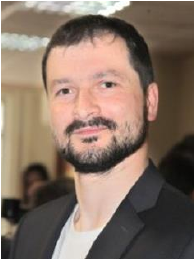
\includegraphics[height=0.25\textheight]{spiros-bond.png}%
    \end{tabular}
    & 
      \begin{tabular}{l}
        \parbox{0.75\linewidth}{%  change the parbox width as appropiate
        \emph{Spiros Bontomitsidis} for his critical comments
        }
      \end{tabular}  \\
  \end{tabular}
  
  \vspace{2em}
 
  
\end{frame}



%%% Local Variables:
%%% mode: latex
%%% TeX-master: "../android-studio-main"
%%% End:


% ================= references =========================

\nocite{*}
\mode*
\appendix
\backupbegin
\begin{frame}[plain, allowframebreaks]
    \frametitle{References}
    \bibliographystyle{abbrvnat}
    {\tiny \bibliography{ref}}
\end{frame}
\backupend

\end{document}




%%% Local Variables:
%%% mode: latex
%%% TeX-master: t
%%% End:
